% The document class supplies options to control rendering of some standard
% features in the result.  The goal is for uniform style, so some attention 
% to detail is *vital* with all fields.  Each field (i.e., text inside the
% curly braces below, so the MEng text inside {MEng} for instance) should 
% take into account the following:
%
% - author name       should be formatted as "FirstName LastName"
%   (not "Initial LastName" for example),
% - supervisor name   should be formatted as "Title FirstName LastName"
%   (where Title is "Dr." or "Prof." for example),
% - degree programme  should be "BSc", "MEng", "MSci", "MSc" or "PhD",
% - dissertation title should be correctly capitalised (plus you can have
%   an optional sub-title if appropriate, or leave this field blank),
% - dissertation type should be formatted as one of the following:
%   * for the MEng degree programme either "enterprise" or "research" to
%     reflect the stream,
%   * for the MSc  degree programme "$X/Y/Z$" for a project deemed to be
%     X%, Y% and Z% of type I, II and III.
% - year              should be formatted as a 4-digit year of submission
%   (so 2014 rather than the accademic year, say 2013/14 say).
%
% Note there is a *strict* requirement for the poster to be in portrait 
% format so that we display them on the poster boards available.

\documentclass[]{templates/poster}

\usepackage{pifont}
\usepackage{caption}
\usepackage{subcaption}
\usepackage{graphicx}

\DeclareGraphicsExtensions{.pdf}

\postertitle{Quantum speedup of the Travelling Salesman Problem for bounded-degree graphs}
\posterauthors{Dominic J. Moylett\textsuperscript{1,2,3}, Noah Linden\textsuperscript{4} and Ashley Montanaro\textsuperscript{4}}
\posteraffils{\textsuperscript{1}Quantum Engineering Technology Labs, University of Bristol\\\textsuperscript{2}Quantum Engineering Centre for Doctoral Training, University of Bristol\\\textsuperscript{3}Heilbronn Institute for Mathematical Research, University of Bristol\\\textsuperscript{4}School of Mathematics, University of Bristol}

\begin{document}

% -----------------------------------------------------------------------------

\begin{frame}{} 

\begin{columns}[t]
  \begin{column}{0.900\linewidth}
  \begin{block}{\Large Introduction}
  The Travelling Salesman Problem (TSP) is one of the oldest and most famous problems in graph theory. As an $NP$-hard problem, it is known that any classical algorithm for exactly solving the problem must take superpolynomial time, otherwise $P = NP$. A na\"ive search across all possible solutions would take an exponential amount of time to solve. Despite this, a number of classical algorithms have been developed to perform better than na\"ive search, including algorithms which solve the TSP for special cases and algorithms which find an approximate solution. But little research has been undertaken on determining whether or not quantum algorithms can outperform classical algorithms for this problem.
  \end{block}
  \end{column}
\end{columns}

\begin{columns}[t]
  \begin{column}{0.422\linewidth}
  \begin{block}{\Large 1. The Travelling Salesman Problem}
  Let $G = (V, E)$ be a graph with $n$ vertices $V$ and $m$ edges $E$. Associated with $G$ is a cost function $C \colon E \rightarrow \mathbb{Z}^+$. A cycle $H$ on $G$ is a {\em Hamiltonian cycle} if it visits every vertex in $G$ exactly once. The Travelling Salesman Problem is defined as follows:
  
  \begin{center}
  ``Given a graph $G$, return the Hamiltonian cycle with minimum cost.''
  \begin{figure}
  \begin{subfigure}[t]{0.3\linewidth}
  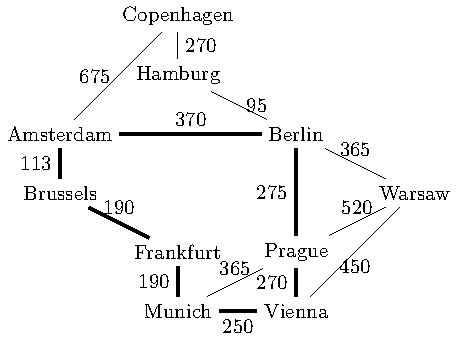
\includegraphics[width=\linewidth]{not_hamiltonian}
  \caption{\ding{55} Not a Hamiltonian cycle.}
  \end{subfigure}
  \begin{subfigure}[t]{0.3\linewidth}
  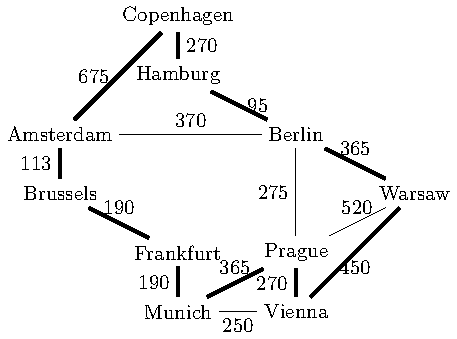
\includegraphics[width=\linewidth]{not_shortest}
  \caption{\ding{55} Not the shortest Hamiltonian cycle. (Length: $2983$ Minutes)}
  \end{subfigure}
  \begin{subfigure}[t]{0.3\linewidth}
  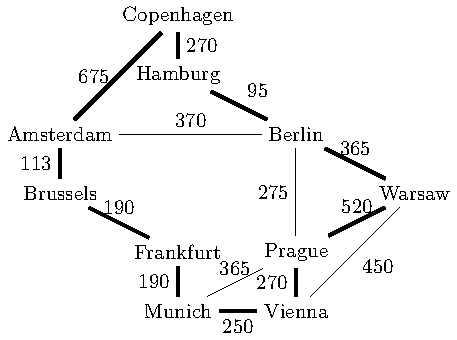
\includegraphics[width=\linewidth]{shortest}
  \caption{\ding{51} Solution to the Travelling Salesman Problem. (Length: $2938$ Minutes)}
  \end{subfigure}
  \end{figure}
  \end{center}
  \end{block}
  \end{column}

  \begin{column}{0.422\linewidth}
  \begin{block}{\Large 2. Our results}
  We demonstrate quadratic speedups for solving the TSP when the degree of any vertex in the graph is at most $4$. This is through applying a quantum speedup for backtracking algorithms developed by Montanaro to a pair of algorithms by Xiao \& Nagamochi for solving the TSP when the maximum degree of any vertex in the graph is $3$ and $4$, respectively. We then demonstrate polynomial speedups for graphs of degrees $5$ and $6$ by reducing these cases to instances of degree-$4$ graphs.
  \end{block}
  \end{column}
\end{columns}

\begin{columns}[t]
  \begin{column}{0.422\linewidth}
  \begin{block}{\Large 3. Backtracking algorithms}
  \end{block}
  \end{column}
  \begin{column}{0.422\linewidth}
  \begin{block}{\Large 4. The Xiao-Nagamochi algorithm for degree-3 graphs}
  \end{block}
  \end{column}
\end{columns}

\begin{columns}[t]
  \begin{column}{0.422\linewidth}
  \begin{block}{\Large 5. Expanding to higher-degree graphs}
  \end{block}
  \end{column}
  \begin{column}{0.422\linewidth}
  \begin{block}{\Large References}
  \end{block}
  \end{column}
\end{columns}

\end{frame}

% -----------------------------------------------------------------------------

\end{document}



